\UseRawInputEncoding
\documentclass[12pt,a4paper]{report}
% ── Packages ──────────────────────────────────────────────────────────────────
\usepackage[utf8]{inputenc}
\usepackage[T1]{fontenc}
\usepackage[french]{babel}
\usepackage{geometry}
\usepackage{graphicx}
\usepackage{xcolor}
\usepackage{fancyhdr}
\usepackage{titlesec}
\usepackage{booktabs}
\usepackage{tabularx}
\usepackage{longtable}
\usepackage{listings}
\usepackage{hyperref}
\usepackage{array}
\usepackage{multirow}
\usepackage{enumitem}
\usepackage{setspace}
\usepackage{microtype}
\usepackage{emptypage}
\usepackage{tcolorbox}
\usepackage{float}
\usepackage{colortbl}
\usepackage{tikz}
\usepackage{needspace}
\usepackage{amssymb}

% ── Géométrie ─────────────────────────────────────────────────────────────────
\geometry{a4paper, top=2.5cm, bottom=2.5cm, left=2.5cm, right=2.5cm}

% ── Couleurs ──────────────────────────────────────────────────────────────────
\definecolor{telecomred}{RGB}{153,0,0}
\definecolor{mainblue}{RGB}{24,95,165}
\definecolor{darkgray}{RGB}{68,68,65}
\definecolor{lightgray}{RGB}{241,239,232}
\definecolor{codegray}{RGB}{44,44,42}
\definecolor{lightblue}{RGB}{230,241,251}
\definecolor{teal}{RGB}{15,110,86}
\definecolor{lightgreen}{RGB}{234,243,222}
\definecolor{lightyellow}{RGB}{255,253,230}
\definecolor{lightorange}{RGB}{250,238,218}

% ── Styles de code ────────────────────────────────────────────────────────────
\lstdefinestyle{bashstyle}{
  backgroundcolor=\color{lightgray},
  basicstyle=\ttfamily\footnotesize\color{codegray},
  breaklines=true,
  literate=
    {é}{{\'e}}1 {è}{{\`e}}1 {ê}{{\^e}}1 {ë}{{\"e}}1
    {à}{{\`a}}1 {â}{{\^a}}1 {ä}{{\"a}}1
    {ù}{{\`u}}1 {û}{{\^u}}1 {ü}{{\"u}}1
    {î}{{\^i}}1 {ï}{{\"i}}1
    {ô}{{\^o}}1 {ö}{{\"o}}1
    {ç}{{\c{c}}}1 {œ}{{\oe}}1 {æ}{{\ae}}1
    {É}{{\'E}}1 {È}{{\`E}}1 {Ê}{{\^E}}1
    {À}{{\`A}}1 {Â}{{\^A}}1
    {Ù}{{\`U}}1 {Û}{{\^U}}1
    {Î}{{\^I}}1 {Ô}{{\^O}}1
    {Ç}{{\c{C}}}1,
  frame=single,
  framerule=0.3pt,
  rulecolor=\color{darkgray!40},
  numbers=none,
  showstringspaces=false,
  tabsize=2,
  xleftmargin=8pt,
  xrightmargin=8pt,
  aboveskip=6pt,
  belowskip=6pt,
}
\lstset{style=bashstyle}

% ── En-têtes et pieds de page ─────────────────────────────────────────────────
\pagestyle{fancy}
\fancyhf{}
\fancyhead[L]{\small\color{darkgray} Projet RAG — Understanding Retrieval-Augmented Generation}
\fancyhead[R]{\small\color{darkgray} Telecom Paris / IP Paris}
\fancyfoot[C]{\small\color{darkgray}\thepage}
\renewcommand{\headrulewidth}{0.4pt}
\renewcommand{\footrulewidth}{0pt}

% ── Styles de titres ──────────────────────────────────────────────────────────
\renewcommand{\contentsname}{Table des matières}
\renewcommand{\listfigurename}{Table des figures}

\titleformat{\chapter}
  {\normalfont\Large\bfseries\color{white}\colorbox{mainblue}}
  {Chapitre \thechapter\ -\ }
  {0pt}
  {}
\titlespacing*{\chapter}{0pt}{0pt}{16pt}

\titleformat{\section}
  {\normalfont\large\bfseries\color{mainblue}}{\thesection}{8pt}{}
\titlespacing*{\section}{0pt}{12pt}{6pt}

\titleformat{\subsection}
  {\normalfont\normalsize\bfseries\color{darkgray}}{\thesubsection}{6pt}{}
\titlespacing*{\subsection}{0pt}{8pt}{4pt}

% ── Boîtes colorées ───────────────────────────────────────────────────────────
\tcbuselibrary{skins,breakable}
\newtcolorbox{infobox}{
  colback=lightblue, colframe=mainblue, boxrule=0.5pt,
  arc=4pt, left=8pt, right=8pt, top=6pt, bottom=6pt, breakable
}
\newtcolorbox{resultbox}{
  colback=lightgreen, colframe=teal, boxrule=0.5pt,
  arc=4pt, left=8pt, right=8pt, top=6pt, bottom=6pt, breakable
}
\newtcolorbox{captionbox}{
  colback=lightyellow, colframe=darkgray!50, boxrule=0.5pt,
  arc=4pt, left=8pt, right=8pt, top=6pt, bottom=6pt, breakable
}
\newtcolorbox{evalbox}{
  colback=lightorange, colframe=teal, boxrule=0.5pt,
  arc=4pt, left=8pt, right=8pt, top=6pt, bottom=6pt, breakable
}

% ── Hyperlinks ────────────────────────────────────────────────────────────────
\hypersetup{
  colorlinks=true, linkcolor=mainblue, urlcolor=mainblue, citecolor=mainblue,
  pdftitle={Rapport RAG — Telecom Paris}, pdfauthor={Leonnel Romuald SOP},
}

% ── Commande capture écran ────────────────────────────────────────────────────
\newcommand{\screenshot}[2]{
  \begin{figure}[H]
    \centering
    \fbox{\begin{minipage}{0.92\textwidth}
      \centering
      \vspace{1.5cm}
      \textcolor{darkgray}{\textit{[Capture d'écran : #1]}}
      \vspace{1.5cm}
    \end{minipage}}
    \caption{#2}
  \end{figure}
}

% ══════════════════════════════════════════════════════════════════════════════
\begin{document}

% ── PAGE DE GARDE ─────────────────────────────────────────────────────────────
\begin{titlepage}
  \thispagestyle{empty}

  \begin{minipage}[t]{0.5\textwidth}
    \vspace{0pt}
    
\includegraphics[width=4cm]{logo_telecom.png}
    \vspace{6pt}

    \textcolor{darkgray}{\rule{5cm}{0.4pt}}
    \vspace{4pt}

    \textbf{\large IP PARIS}
  \end{minipage}
  \hfill
  \begin{minipage}[t]{0.45\textwidth}
    \vspace{0pt}
    \raggedleft
    \textbf{\large\color{telecomred} ANNEE 2025/2026}
  \end{minipage}

  \vspace{3cm}

  \begin{center}
    {\Large\bfseries PROJECT RAG}
    \vspace{1.5cm}

    \textit{\large Thématique :}
    \vspace{0.4cm}

    \begin{tcolorbox}[
      colback=lightgray, colframe=darkgray!50,
      boxrule=0.5pt, arc=4pt, width=\textwidth
    ]
      \begin{center}
        {\LARGE\bfseries\color{mainblue}
          Understanding Retrieval-Augmented\\[6pt]
          Generation (RAG)
        }
      \end{center}
    \end{tcolorbox}
  \end{center}

  \vspace{2cm}

  \begin{center}
  \begin{tabular}{rl}
    \textbf{Étudiant :}    & Leonnel Romuald SOP \\[6pt]
    \textbf{Professeur :}  & Julien Dreano \\[6pt]
    \textbf{Contact :}     & \texttt{julien.dreano@gmail.com} \\[6pt]
    \textbf{Année :}       & 2025/2026 \\
  \end{tabular}
  \end{center}

  \vspace{1cm}
  \begin{center}
    \textcolor{darkgray}{\rule{10cm}{0.4pt}}
  \end{center}
  \vspace{0.6cm}

\end{titlepage}

% ── TABLE DES MATIÈRES ────────────────────────────────────────────────────────
\tableofcontents
\newpage

% ── TABLE DES FIGURES ─────────────────────────────────────────────────────────
\listoffigures
\newpage

% ══════════════════════════════════════════════════════════════════════════════
\chapter{Description de l'environnement}

\section{Machine hôte}

La machine hôte utilisée pour ce projet est un poste de travail personnel équipé
d'un processeur \textbf{AMD Ryzen 7}, d'une carte graphique \textbf{NVIDIA RTX 4090}
et de \textbf{32 Go de RAM}, fonctionnant sous \textbf{Windows 11}.

\section{Machine virtuelle}

Conformément à la consigne, une machine virtuelle Linux a été déployée via
\textbf{VMware Workstation}. La distribution choisie est \textbf{Ubuntu 22.04 LTS},
configurée avec 8 Go de RAM et 100 Go de stockage. Ollama fonctionne en mode CPU
à l'intérieur de la VM, le GPU physique n'étant pas accessible via VMware Workstation
sous Windows.

\begin{infobox}
\textbf{Note importante :} VMware Workstation sous Windows ne supporte pas le GPU
passthrough pour les GPU NVIDIA grand public. La RTX 4090 reste donc inaccessible
depuis la VM — Ollama bascule automatiquement en mode CPU (40 à 190 secondes par
réponse). Cette limitation est documentée en section 8.2.
\end{infobox}

\vspace{8pt}

  \begin{center}
  \small
  \begin{tabular}{|l|l|l|}
    \hline
    \rowcolor{mainblue}
    \textcolor{white}{\textbf{Composant}} &
    \textcolor{white}{\textbf{Technologie}} &
    \textcolor{white}{\textbf{Version}} \\
    \hline
    LLM local          & Ollama — llama3.1:8b              & 0.30.10 \\
    \rowcolor{lightblue}
    Embedding          & nomic-embed-text (Ollama)         & — \\
    Base vectorielle   & PostgreSQL + pgvector             & 16 / 0.8.3 \\
    \rowcolor{lightblue}
    Orchestration      & LangChain Python                  & 0.3.25 \\
    Conteneurisation   & Docker Compose                    & 5.1.4 \\
    \rowcolor{lightblue}
    Dataset            & neural-bridge/rag-dataset-12000   & 9~600 entrées \\
    VM                 & Ubuntu 22.04 — VMware Workstation & — \\
    \hline
  \end{tabular}
  \end{center}

% ══════════════════════════════════════════════════════════════════════════════
\chapter{Processus d'installation}

\section{Vérification de l'environnement}

Avant de démarrer, on vérifie que Docker et Ollama sont bien installés et
opérationnels dans la VM :

\begin{lstlisting}[language=bash]
# Verification Docker
docker --version
docker compose version

# Verification Ollama
ollama --version
ollama list
\end{lstlisting}

\begin{figure}[H]
  \centering
  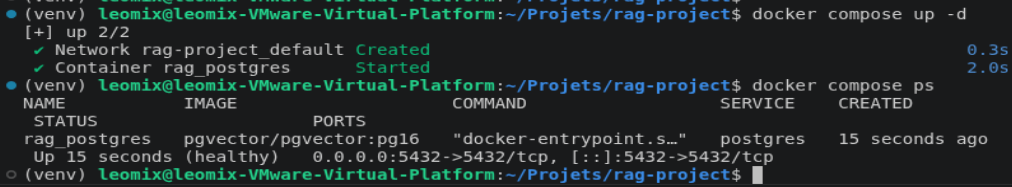
\includegraphics[width=1\textwidth]{Capture 1 — Docker.png}
  \caption{Vérification de l'environnement}
  \label{fig:Environ}
\end{figure}


\section{Création et activation du virtualenv Python}

Le virtualenv isole les dépendances du projet du système Python global :

\begin{lstlisting}[language=bash]
# Creation du venv
python3 -m venv /home/leomix/Projets/rag-project/venv

# Activation
source /home/leomix/Projets/rag-project/venv/bin/activate

# Verification : doit afficher le chemin du venv
which pip
\end{lstlisting}

\section{Configuration du fichier d'environnement (\texttt{.env})}

Les scripts Python utilisent \texttt{python-dotenv} pour lire leurs paramètres
de connexion depuis un fichier \texttt{.env} situé à la racine du projet.
Ce fichier doit être créé avant de lancer les scripts :

\begin{lstlisting}[language=bash]
cat > /home/leomix/Projets/rag-project/.env << EOF
DB_HOST=localhost
DB_PORT=5432
DB_NAME=rag_db
DB_USER=rag_user
DB_PASSWORD=rag_password
OLLAMA_BASE_URL=http://localhost:11434
EOF
\end{lstlisting}

\begin{infobox}
\textbf{Note :} Ces valeurs correspondent aux paramètres par défaut définis dans
\texttt{compose.yml}. En l'absence du fichier \texttt{.env}, les scripts utilisent
automatiquement ces valeurs par défaut — le fichier est donc optionnel mais recommandé
pour faciliter la maintenance et éviter de coder les credentials en dur.
\end{infobox}

\section{Installation des dépendances Python}

\begin{lstlisting}[language=bash]
pip install -r requirements.txt
\end{lstlisting}

Les librairies principales installées sont : \texttt{langchain}, \texttt{langchain-ollama},
\texttt{psycopg2-binary}, \texttt{pgvector}, \texttt{datasets}, \texttt{rouge-score},
\texttt{bert-score} et \texttt{deep-translator}.

\section{Pull des modèles Ollama}

Deux modèles sont nécessaires — un pour la génération de texte, un pour l'embedding.
Le modèle \textbf{llama3.1:8b} a été retenu pour ses performances multilingues et sa
taille adaptée au mode CPU (4,9 Go, contexte 128k tokens) ; \textbf{nomic-embed-text}
pour ses vecteurs 768 dimensions compacts et de haute qualité sémantique :

\begin{lstlisting}[language=bash]
# Modele LLM principal (4.9 Go)
ollama pull llama3.1:8b

# Modele d'embedding (274 Mo - 768 dimensions)
ollama pull nomic-embed-text

# Verification
ollama list
\end{lstlisting}

\begin{figure}[H]
  \centering
  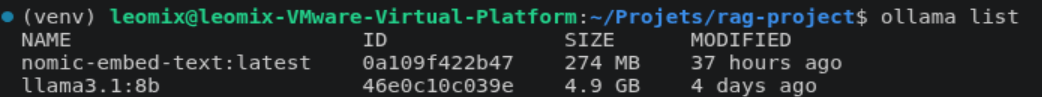
\includegraphics[width=1\textwidth]{Capture 3 — Ollama.png}
  \caption{Modèles Ollama disponibles}
  \label{fig:ollama}
\end{figure}

\section{Déploiement PostgreSQL + pgvector via Docker}

PostgreSQL est déployé dans un conteneur Docker avec l'extension pgvector
pré-installée via l'image officielle \texttt{pgvector/pgvector:pg16} :

\begin{lstlisting}[language=bash]
# Lancement du conteneur en arriere-plan
cd /home/leomix/Projets/rag-project
docker compose up -d

# Verification du statut (doit afficher "healthy")
docker compose ps

# Verification de l'extension pgvector
docker exec -it rag_postgres psql -U rag_user -d rag_db \
  -c "SELECT extname, extversion FROM pg_extension WHERE extname='vector';"
\end{lstlisting}



\begin{figure}[H]
  \centering
  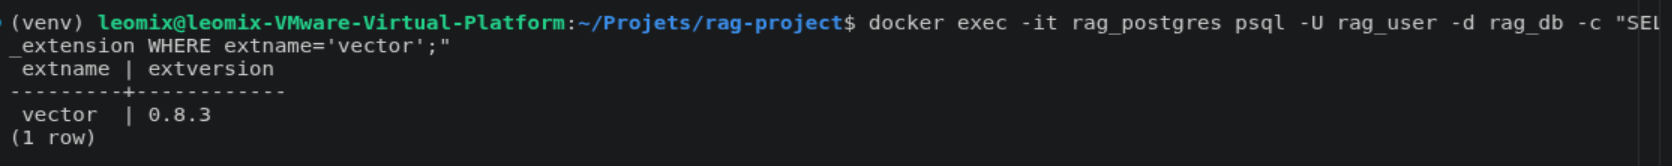
\includegraphics[width=1\textwidth]{Capture 9 — deploiement.png}
  \caption{\textbf{Déploiement PostgreSQL + pgvector:} Terminal montrant docker compose ps avec le statut healthy et
la requête SQL retournant vector 0.8.3}
  \label{fig:requete}
\end{figure}

\begin{resultbox}
\textbf{Résultat attendu :}
\begin{verbatim}
 extname | extversion
---------+------------
 vector  | 0.8.3
\end{verbatim}
\end{resultbox}

% ══════════════════════════════════════════════════════════════════════════════
\chapter{Architecture de l'environnement}

L'environnement est structuré en trois couches superposées : la machine hôte Windows,
la VM Ubuntu gérée par VMware, et à l'intérieur de cette VM, les composants applicatifs.

\vspace{8pt}
\begin{center}
\begin{tabular}{|l|l|l|}
  \hline
  \rowcolor{mainblue}
  \textcolor{white}{\textbf{Couche}} &
  \textcolor{white}{\textbf{Composant}} &
  \textcolor{white}{\textbf{Rôle}} \\
  \hline
  Machine hôte        & Windows 11 / RTX 4090         & Hôte physique \\
  \rowcolor{lightblue}
  Virtualisation      & VMware Workstation            & Isolation de l'environnement \\
  OS invité           & Ubuntu 22.04 LTS              & Système d'exploitation du projet \\
  \rowcolor{lightblue}
  LLM                 & Ollama (llama3.1:8b)          & Génération de réponses \\
  Embedding           & nomic-embed-text              & Vectorisation des textes \\
  \rowcolor{lightblue}
  Base vectorielle    & PostgreSQL + pgvector         & Stockage et recherche de vecteurs \\
  Conteneur           & Docker Compose                & Isolation de PostgreSQL \\
  \rowcolor{lightblue}
  Orchestration       & LangChain Python              & Pipeline RAG end-to-end \\
  Dataset             & HuggingFace (9~600 docs)      & Base de connaissance RAG \\
  \hline
\end{tabular}
\end{center}

\section{Schéma architecture de l'environnement}

Le schéma ci-dessous illustre les trois couches de l'environnement et les
interactions entre les composants. Les flèches montrent les flux de données :
les scripts Python appellent Ollama (port 11434) pour générer les embeddings
et les réponses LLM, et PostgreSQL (port 5432) pour stocker et rechercher
les vecteurs.

\begin{infobox}
\textbf{Interactions clés :}
\begin{itemize}[leftmargin=1cm]
  \item \textbf{Python $\rightarrow$ Ollama (port 11434)} : génération des embeddings
        (nomic-embed-text) et des réponses LLM (llama3.1:8b)
  \item \textbf{Python $\rightarrow$ PostgreSQL (port 5432)} : stockage et recherche
        vectorielle via pgvector
  \item \textbf{HuggingFace $\rightarrow$ Python} : téléchargement automatique du
        dataset au premier lancement de \texttt{ingest.py}
\end{itemize}
\end{infobox}

\vspace{6pt}

\begin{figure}[H]
  \centering
  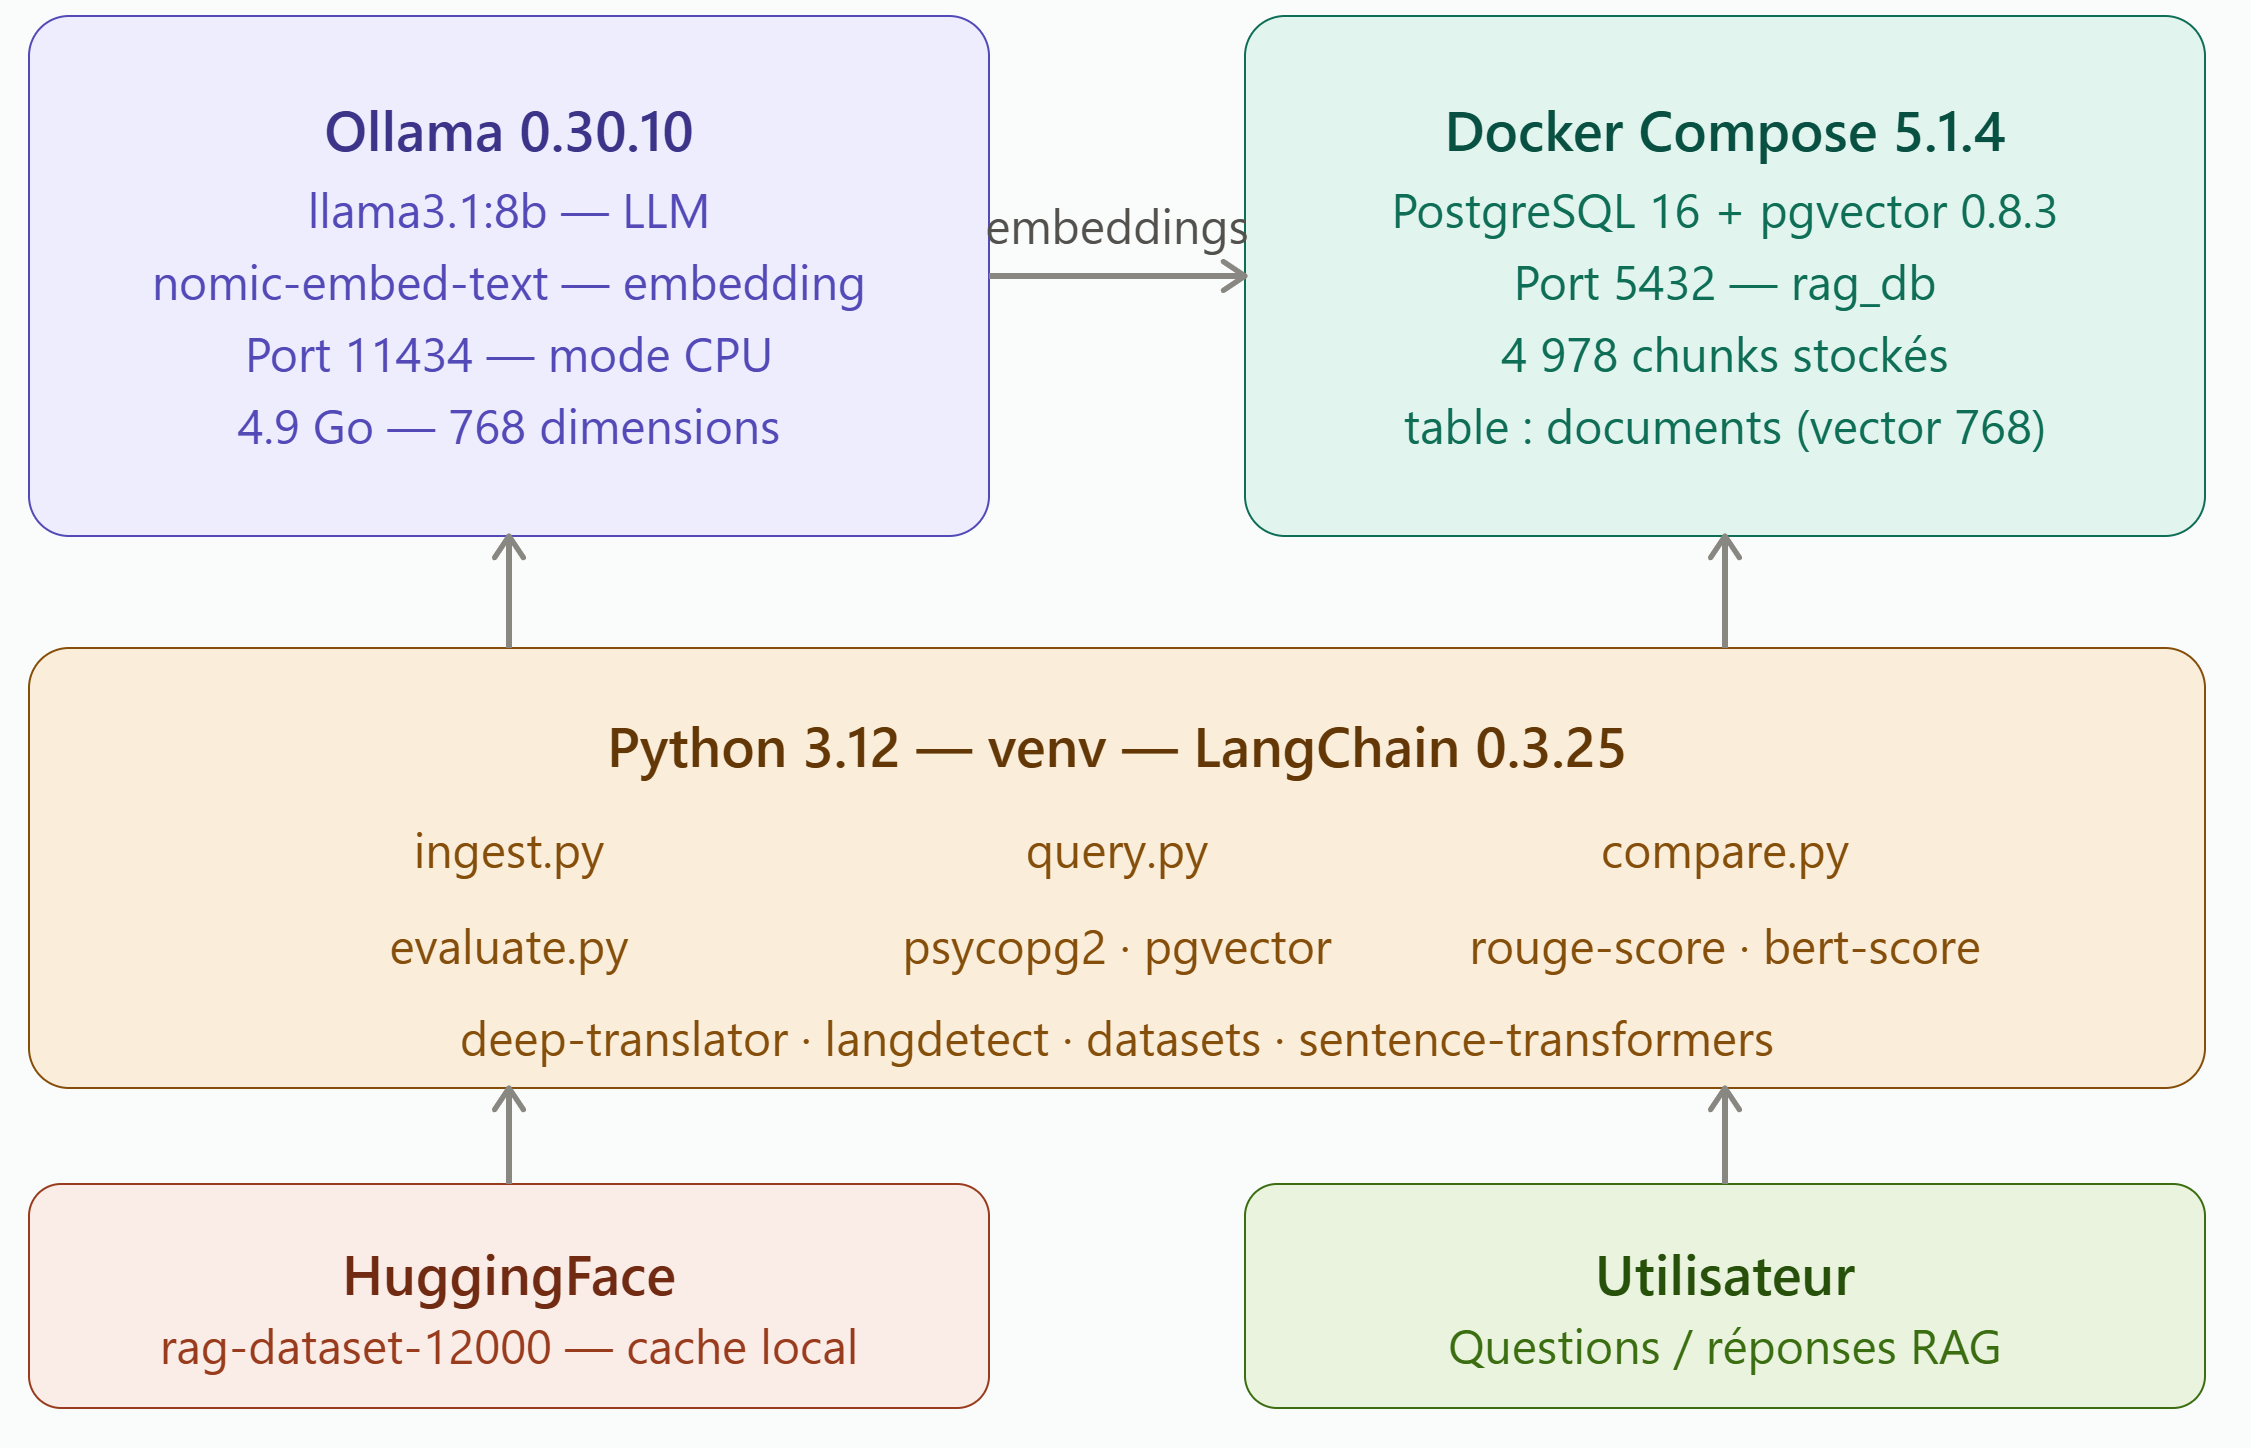
\includegraphics[width=0.8\textwidth]{architecture_rag_stylise.png}
  \caption{Architecture complète de l'environnement RAG — trois couches :
  machine hôte Windows, VM Ubuntu VMware, composants applicatifs}
  \label{fig:architecture}
\end{figure}

% ══════════════════════════════════════════════════════════════════════════════
\chapter{Pipeline RAG: Workflow complet}

Le pipeline RAG se décompose en deux sous-pipelines distincts : l'ingestion des
documents et l'interrogation du LLM. Le schéma ci-dessous présente la vue
d'ensemble du workflow complet.

\begin{figure}[H]
  \centering
  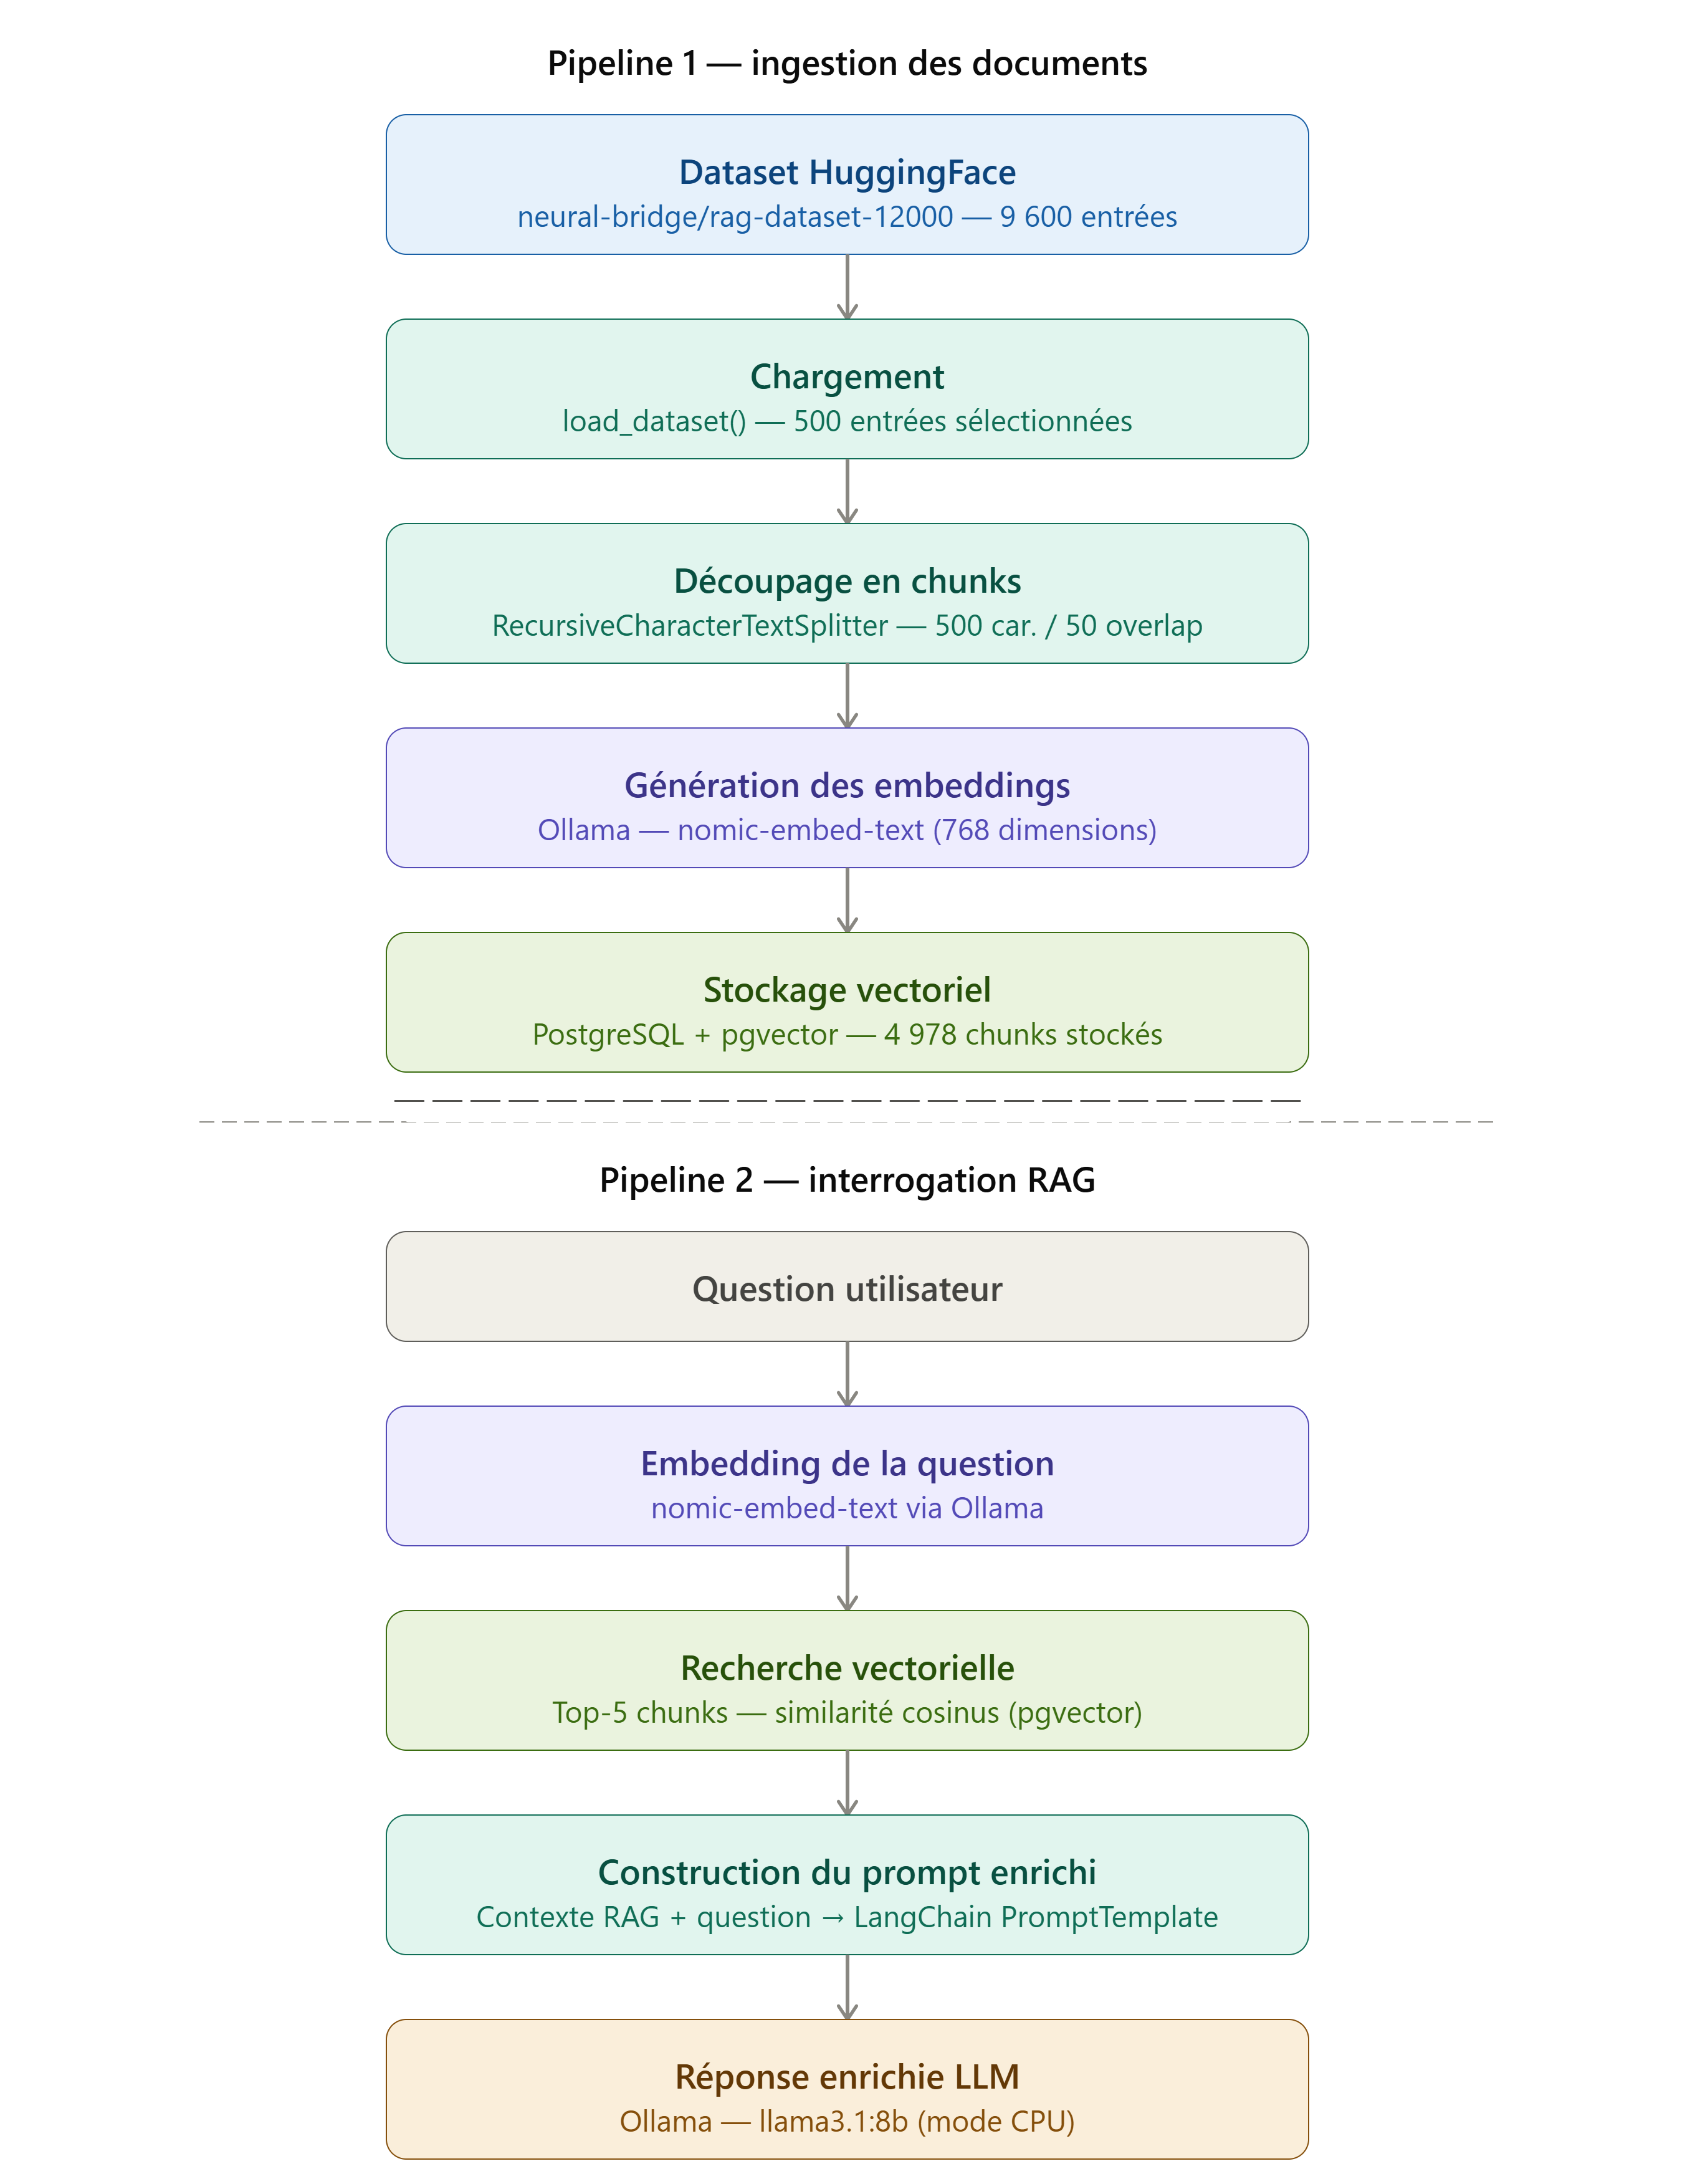
\includegraphics[width=1\textwidth]{workflow_rag_stylise.png}
  \caption{Workflow RAG complet — Pipeline 1 : ingestion des documents /
  Pipeline 2 : interrogation du LLM}
  \label{fig:Workflow}
\end{figure}

\section{Pipeline 1 — Ingestion des documents}

L'ingestion transforme le dataset brut en vecteurs stockés dans pgvector.
Elle se déroule en 5 étapes séquentielles :

\subsection{Étape 1 — Chargement du dataset HuggingFace}

La librairie \texttt{datasets} télécharge automatiquement le dataset au premier
lancement et le met en cache localement pour les lancements suivants :

\begin{lstlisting}[language=Python]
dataset = load_dataset('neural-bridge/rag-dataset-12000', split='train')
entries = dataset.select(range(500))  # 500 entrees sur 9600
\end{lstlisting}

\begin{captionbox}
\textbf{Pourquoi 500 entrées sur 9~600 ?} Chaque entrée génère en moyenne 10 chunks
après découpage. 500 entrées $\times$ 10 chunks = 4~978 chunks stockés. Ingérer
les 9~600 aurait pris plusieurs heures en mode CPU. Pour ingérer l'intégralité
du dataset, deux approches sont envisageables : lancer \texttt{ingest.py} en tâche
de fond pendant la nuit (\texttt{nohup python3 ingest.py \&}), ou utiliser un
environnement avec GPU via WSL2 plutôt que VMware.
\end{captionbox}

\subsection{Étape 2 — Découpage en chunks (chunking)}

Les textes longs sont découpés en morceaux exploitables par le LLM.
\texttt{RecursiveCharacterTextSplitter} découpe en respectant la hiérarchie
naturelle du texte : paragraphes $\rightarrow$ lignes $\rightarrow$ phrases
$\rightarrow$ mots :

\begin{lstlisting}[language=Python]
splitter = RecursiveCharacterTextSplitter(
    chunk_size=500,    # max 500 caracteres par chunk
    chunk_overlap=50   # 50 caracteres de chevauchement
)
splits = splitter.split_text(context)
\end{lstlisting}

Le chevauchement de 50 caractères garantit qu'une information à cheval
sur deux chunks ne soit pas perdue.

\subsection{Étape 3 — Génération des embeddings}

Chaque chunk est transformé en vecteur de 768 dimensions par
\texttt{nomic-embed-text} via Ollama. Ce vecteur capture le sens sémantique
du texte — deux textes qui parlent du même sujet auront des vecteurs proches,
même s'ils n'ont pas un seul mot en commun :

\begin{lstlisting}[language=Python]
embeddings_model = OllamaEmbeddings(
    model='nomic-embed-text',
    base_url='http://localhost:11434'
)
vectors = embeddings_model.embed_documents(texts)
# Chaque vecteur = liste de 768 nombres flottants
\end{lstlisting}

\subsection{Étape 4 — Stockage dans pgvector}

Les chunks et leurs vecteurs sont insérés dans la table \texttt{documents}
de PostgreSQL par lots de 20 pour optimiser les performances :


\begin{figure}[H]
  \centering
  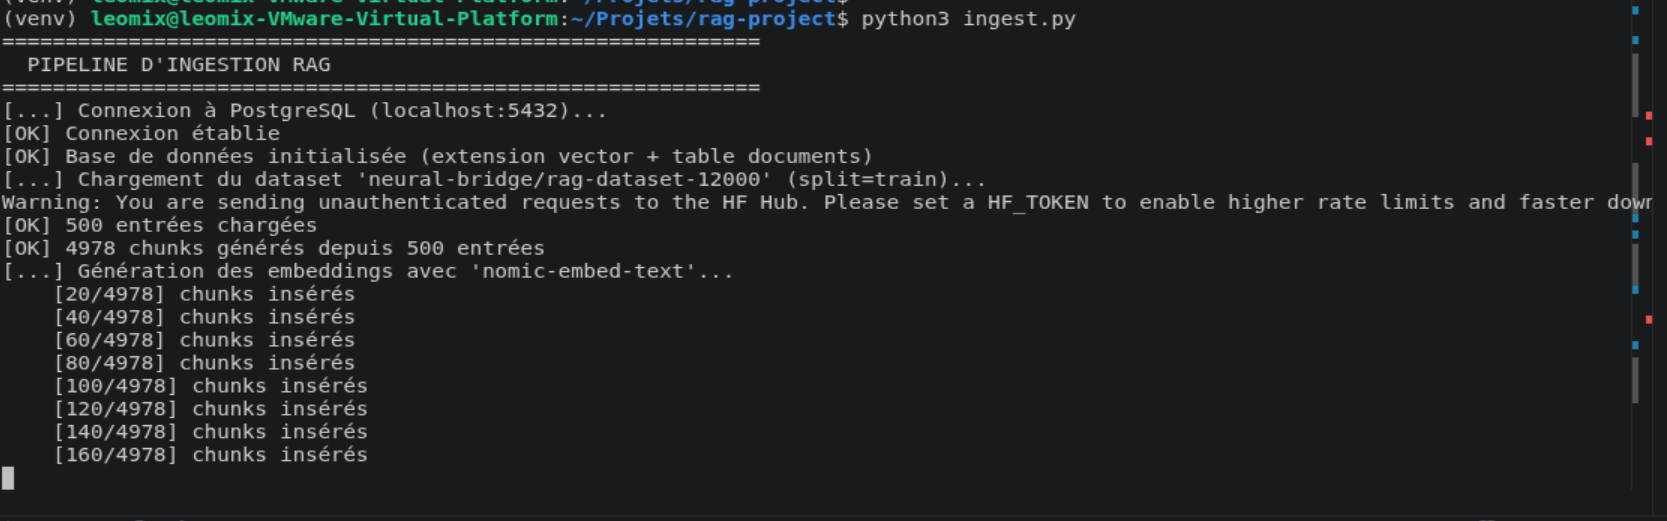
\includegraphics[width=1\textwidth]{Capture 4 — Ingestion.png}
  \caption{Pipeline d'ingestion RAG — début de l'ingestion}
  \label{fig:ingestion}
\end{figure}


\subsection{Résultat de l'ingestion}

\begin{figure}[H]
  \centering
  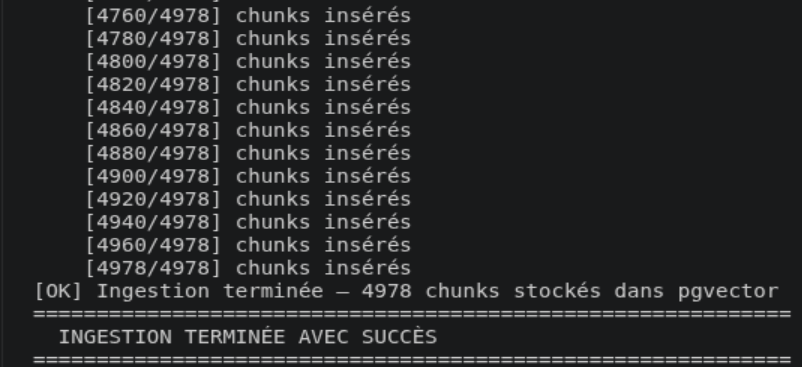
\includegraphics[width=1\textwidth]{Capture 4-1 — Ingestion.png}
  \caption{Fin de l'ingestion avec 4 978 chunks stockés dans pgvector}
  \label{fig:pgvector}
\end{figure}

\begin{lstlisting}[language=bash]
# Verification en base
docker exec -it rag_postgres psql -U rag_user -d rag_db \
  -c "SELECT COUNT(*) FROM documents;"
\end{lstlisting}

\begin{figure}[H]
  \centering
  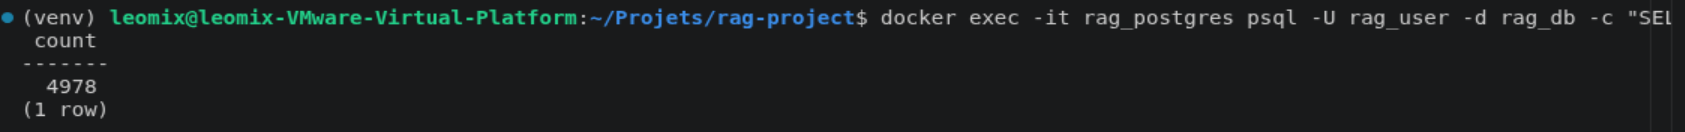
\includegraphics[width=1\textwidth]{Capture 5 — Vérification base.png}
  \caption{Confirmation des 4 978 chunks en base PostgreSQL}
  \label{fig:verif}
\end{figure}

\begin{resultbox}
\textbf{Résultat ingestion :} 500 entrées chargées $\rightarrow$
4~978 chunks générés $\rightarrow$ 4~978 vecteurs (768D) stockés dans pgvector.
\end{resultbox}

\section{Pipeline 2 — Interrogation RAG}

L'interrogation transforme une question en réponse enrichie par le contexte.
Elle se déroule en 4 étapes :

\subsection{Étape 1 — Embedding de la question}

La question est transformée en vecteur 768D par le même modèle
\texttt{nomic-embed-text} utilisé lors de l'ingestion. Cela garantit
que les vecteurs sont comparables dans le même espace sémantique :

\begin{lstlisting}[language=Python]
query_embedding = embeddings_model.embed_query(question)
# question (texte) -> vecteur 768 dimensions
\end{lstlisting}

\subsection{Étape 2 — Recherche vectorielle dans pgvector}

pgvector calcule la distance cosinus entre le vecteur de la question
et les 4~978 vecteurs stockés. Les 5 chunks les plus proches
sémantiquement sont retournés :

\begin{lstlisting}[language=Python]
cur.execute("""
    SELECT content, source,
           1 - (embedding <=> %s::vector) AS similarity
    FROM documents
    ORDER BY embedding <=> %s::vector
    LIMIT 5;
""", (query_embedding, query_embedding))
\end{lstlisting}

L'opérateur \texttt{<=>} est la distance cosinus propre à pgvector.
\texttt{1 - distance} donne le score de similarité : 1 = identique, 0 = aucun lien.

\subsection{Étape 3 — Construction du prompt enrichi}

Les 5 chunks pertinents sont assemblés en un contexte injecté dans
le prompt avant la question. Le LLM est ainsi contraint de répondre
en se basant uniquement sur ces documents :

\begin{lstlisting}[language=Python]
RAG_PROMPT = """
Tu es un assistant intelligent. Utilise uniquement le contexte
fourni ci-dessous pour repondre a la question. Si le contexte
ne contient pas l'information necessaire, dis-le clairement.

Contexte :
{context}    <- les 5 chunks pertinents

Question : {question}

Reponse :"""
\end{lstlisting}

\begin{captionbox}
\textbf{Pourquoi un prompt en français ?} Le template RAG est rédigé en français
pour contraindre \texttt{llama3.1:8b} à générer ses réponses dans cette langue,
quelle que soit la langue de la question. Le dataset \texttt{neural-bridge/rag-dataset-12000}
étant en anglais, llama3.1:8b répond nativement en anglais si le prompt ne précise
pas la langue. Ce choix explique les réponses en français observées même pour
des questions posées en anglais — et justifie la traduction automatique de la
référence dans \texttt{evaluate.py} pour des métriques ROUGE/BLEU comparables.
\end{captionbox}

\subsection{Étape 4 — Génération de la réponse par llama3.1:8b}

Le prompt enrichi est envoyé à Ollama qui fait tourner llama3.1:8b
localement. Le modèle lit le contexte, identifie les passages pertinents
et génère une réponse précise sans hallucination :

\begin{lstlisting}[language=Python]
llm = OllamaLLM(model='llama3.1:8b', base_url='http://localhost:11434')
response = llm.invoke(prompt)
\end{lstlisting}

\begin{figure}[H]
  \centering
  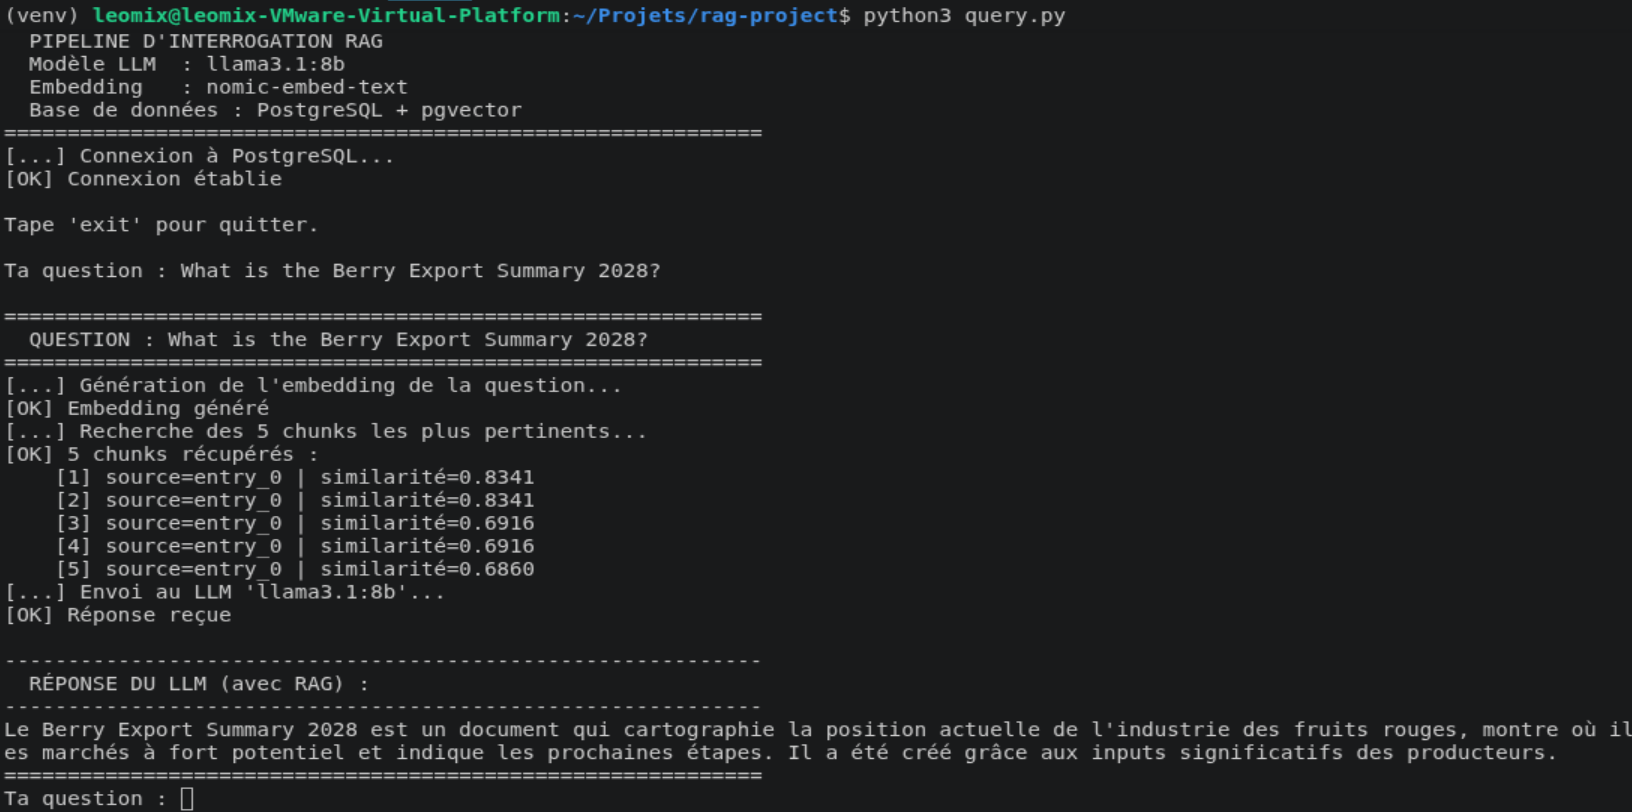
\includegraphics[width=1\textwidth]{Capture 6 — query.py.png}
  \caption{Terminal affichant une session complète de query.py :
question posée, 5 chunks récupérés avec scores de similarité,
réponse du LLM}
  \label{fig:query}
\end{figure}


% ══════════════════════════════════════════════════════════════════════════════
\chapter{Scripts Python développés}

\section{ingest.py — Pipeline d'ingestion}

Ce script réalise le pipeline complet d'ingestion en autonomie : il
télécharge le dataset, découpe les textes, génère les embeddings et
stocke les vecteurs dans pgvector sans aucune intervention manuelle.

\begin{lstlisting}[language=bash]
python3 ingest.py
\end{lstlisting}

\begin{captionbox}
\textbf{À lancer une seule fois.} Les 4~978 chunks survivent aux
redémarrages grâce au volume Docker. Ne relancer que si la base est vidée.
\end{captionbox}

\section{query.py — Interrogation RAG interactive}

Script interactif qui interroge le LLM enrichi par la base de connaissance RAG.
Pour chaque question tapée, il affiche les scores de similarité des chunks
récupérés et la réponse du LLM.

\begin{lstlisting}[language=bash]
python3 query.py
# -> Tape ta question
# -> Reponse RAG + similarites affichees
# -> Tape 'exit' pour quitter
\end{lstlisting}

\section{compare.py — Comparaison RAG vs sans RAG (temps réel)}

Script interactif qui génère en temps réel deux réponses pour chaque question :
une sans RAG (LLM seul basé sur ses données d'entraînement) et une avec RAG
(LLM enrichi par le contexte pgvector), affichées côte à côte.

\begin{lstlisting}[language=bash]
python3 compare.py
# -> Tape ta question
# -> Reponse SANS RAG affichee (avec temps)
# -> Reponse AVEC RAG affichee (avec temps + similarite)
# -> Difference clee mise en evidence
\end{lstlisting}

\begin{figure}[H]
  \centering
  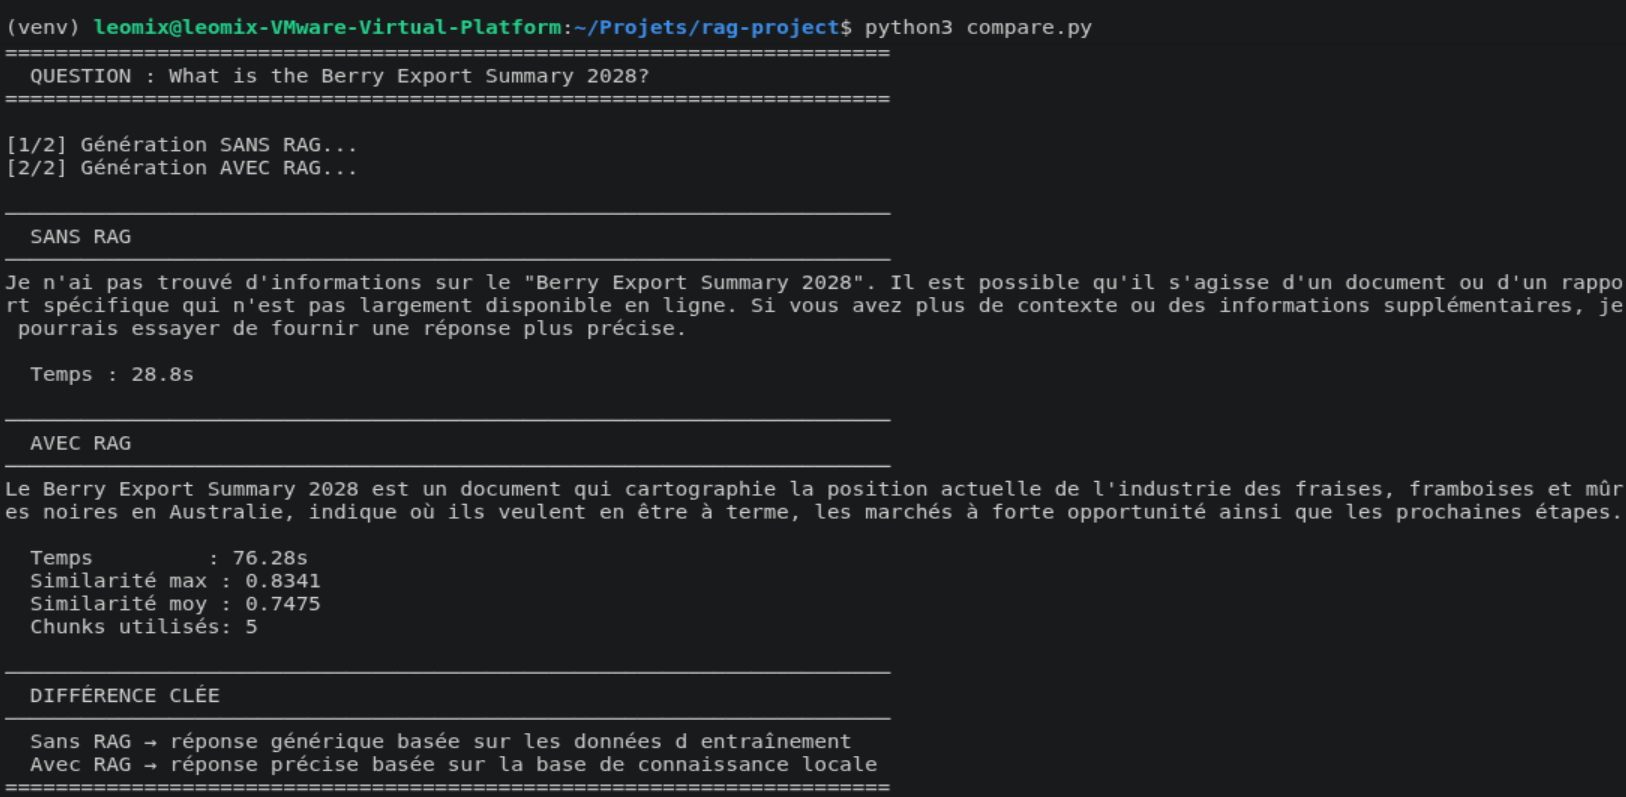
\includegraphics[width=1\textwidth]{Capture 7 — compare.py.png}
  \caption{Terminal affichant une session compare.py avec deux réponses
côte à côte pour la question "What is the Berry Export Summary 2028?" :
sans RAG (vague, 155s) vs avec RAG (précise, 68s)}
  \label{fig:compare}
\end{figure}

\section{evaluate.py — Évaluateur de métriques (temps réel)}

Script interactif qui évalue la qualité des réponses RAG avec 7 métriques.
La référence est automatiquement traduite dans la langue de la réponse via
\texttt{deep-translator} pour garantir des scores fiables quelle que soit
la langue utilisée.

\begin{lstlisting}[language=Python]
# Detection automatique de la langue de la reponse
response_lang = detect_language(response)

# Traduction de la reference dans la meme langue
reference_aligned = translate_to(reference, response_lang)

# Calcul des metriques
rouge = compute_rouge(response, reference_aligned)
bleu  = compute_bleu(response, reference_aligned)
bert  = compute_bertscore(response, reference_aligned)
\end{lstlisting}

\section{generate\_schemas.py — Génération des schémas du rapport}

Ce script utilitaire génère automatiquement les deux schémas du rapport au
format PNG grâce à la librairie \texttt{matplotlib}. Il a été utilisé comme
base de conception des figures LaTeX intégrées dans ce document.

\begin{lstlisting}[language=bash]
python3 generate_schemas.py
# -> rapport/schemas/workflow_rag.png
# -> rapport/schemas/architecture_env.png
\end{lstlisting}

\begin{captionbox}
\textbf{Usage :} Les schémas PNG générés ont servi de prototype visuel ; les
figures finales du rapport (Fig.~\ref{fig:architecture} et Fig.~\ref{fig:Workflow})
ont été retravaillées directement en LaTeX pour s'intégrer à la mise en page
du document.
\end{captionbox}

% ══════════════════════════════════════════════════════════════════════════════
\chapter{Tableau prompt / réponse RAG}

Le tableau ci-dessous présente 6 questions posées au LLM enrichi via la base de
connaissance RAG. Les réponses, issues des chunks récupérés par pgvector, démontrent
que le modèle s'appuie sur des données factuelles précises du dataset plutôt que
sur sa mémoire générale — ce que confirment les scores de similarité max élevés.

\vspace{8pt}
\begin{center}
\small
\begin{tabular}{|c|p{4cm}|p{7cm}|c|}
  \hline
  \rowcolor{mainblue}
  \textcolor{white}{\textbf{\#}} &
  \textcolor{white}{\textbf{Question (prompt)}} &
  \textcolor{white}{\textbf{Réponse LLM (RAG)}} &
  \textcolor{white}{\textbf{Sim. max}} \\
  \hline
  1 & What is the Berry Export Summary 2028 and what is its purpose? &
      Le Berry Export Summary 2028 cartographie la position actuelle des secteurs
      d'exportation australiens de framboises, fraises et myrtilles. Son objectif est
      d'identifier les marchés à fort potentiel et d'établir une stratégie de
      croissance internationale sur 10 ans. & 0.825 \\
  \rowcolor{lightblue}
  2 & Best short-term markets for blackberry/raspberry industry? &
      Les meilleurs marchés à court terme sont Hong Kong, Singapour, les Émirats
      arabes unis et le Canada. Ces marchés ont été identifiés comme prioritaires
      en raison de leur demande croissante pour les fruits rouges australiens. & 0.876 \\
  3 & Role of Hort Innovation in the berry export strategy? &
      Hort Innovation a commandité ce projet et détermine les activités financées
      pour soutenir les échanges commerciaux. Elle joue un rôle central de
      coordination et de financement dans la mise en œuvre de la stratégie
      d'exportation. & 0.830 \\
  \rowcolor{lightblue}
  4 & How much did exports grow between 2016 and 2017? &
      La valeur et le volume des exportations australiennes de fruits rouges ont
      augmenté de 100\% entre 2016 et 2017, passant d'environ 2~000 à plus de
      4~000 tonnes. Cette croissance exponentielle justifie l'élaboration d'un
      plan stratégique sur 10 ans. & 0.877 \\
  5 & Strawberry export target by volume? &
      Le secteur des fraises vise à doubler sa part d'exportation de 4\% à 8\%
      du volume national. Cet objectif ambitieux fait partie du plan de
      développement international décrit dans le Berry Export Summary 2028. & 0.854 \\
  \rowcolor{lightblue}
  6 & Percentage boost for raspberries by 2021? &
      Les secteurs de framboises et mûres visent une augmentation de 5\% en volume
      dans les marchés identifiés d'ici 2021. Cet objectif s'inscrit dans la
      stratégie globale d'expansion des exportations australiennes de fruits
      rouges. & 0.869 \\
  \hline
\end{tabular}
\end{center}

\begin{captionbox}
\textbf{Lecture du tableau :} La colonne \textit{Sim. max} indique le score de
similarité cosinus du chunk le plus pertinent récupéré par pgvector (1 = identique,
0 = aucun lien sémantique). Un score $>$ 0.80 confirme que pgvector a bien retrouvé
le passage source correspondant à la question. Les réponses contenant des données
chiffrées précises (100\%, 4\%, 8\%, 5\%) proviennent directement des chunks
récupérés et ne peuvent pas être générées par le LLM seul sans le RAG.
\end{captionbox}

% ══════════════════════════════════════════════════════════════════════════════
\chapter{Comparaison RAG vs sans RAG}

Le script \texttt{compare.py} permet de comparer en temps réel les réponses avec
et sans RAG pour n'importe quelle question tapée par l'utilisateur.

\vspace{8pt}
\begin{center}
\small
\begin{tabular}{|c|p{3cm}|p{3.5cm}|p{3.5cm}|c|}
  \hline
  \rowcolor{mainblue}
  \textcolor{white}{\textbf{\#}} &
  \textcolor{white}{\textbf{Question}} &
  \textcolor{white}{\textbf{Sans RAG}} &
  \textcolor{white}{\textbf{Avec RAG}} &
  \textcolor{white}{\textbf{Sim.}} \\
  \hline
  1 & Berry Export Summary? &
      Vague / générique (155s) &
      Précise et documentée (68s) & 0.825 \\
  \rowcolor{lightblue}
  2 & Best short-term markets? &
      \textcolor{telecomred}{Inventé (Chine, Japon) (80s)} &
      \textcolor{teal}{Exact (HK, SG, UAE, CA) (42s)} & 0.876 \\
  3 & Export growth 2016-2017? &
      \textcolor{telecomred}{Inventé (3-4\% FAO) (52s)} &
      \textcolor{teal}{Exact (100\%) (40s)} & 0.877 \\
  \rowcolor{lightblue}
  4 & Strawberry target? &
      Pas de réponse (19s) &
      \textcolor{teal}{Exact (4\% $\rightarrow$ 8\%) (38s)} & 0.854 \\
  5 & Tonnes exported? &
      Pas de réponse (27s) &
      \textcolor{teal}{Exact (4244t) (29s)} & 0.795 \\
  \rowcolor{lightblue}
  6 & Price per kg? (piège) &
      Évasif (39s) &
      Honnête — info absente (38s) & 0.749 \\
  7 & Who signed? (piège) &
      Pas de réponse (15s) &
      Honnête — info absente (35s) & 0.763 \\
  \hline
\end{tabular}
\end{center}

\vspace{8pt}
\begin{infobox}
\textbf{Trois enseignements clés :}
\begin{itemize}[leftmargin=1cm]
  \item \textbf{Élimination des hallucinations (Q2, Q3)} : sans RAG le LLM invente
        des marchés inexistants (Chine, Japon) et des chiffres FAO erronés.
        Avec RAG il cite exactement les données du dataset.
  \item \textbf{Précision accrue (Q1, Q4, Q5)} : le RAG fournit des réponses
        factuelles précises là où le LLM seul est vague ou silencieux.
  \item \textbf{Honnêteté sur les questions hors scope (Q6, Q7)} : le RAG
        explique précisément pourquoi il ne peut pas répondre
        (information absente du contexte) plutôt que d'inventer.
\end{itemize}
\end{infobox}

% ══════════════════════════════════════════════════════════════════════════════
\chapter{Métriques d'évaluation}

\section{Présentation des métriques}

Le script \texttt{evaluate.py} évalue la qualité des réponses RAG avec
7 métriques complémentaires sur \textbf{3 questions distinctes}. La référence
est automatiquement traduite dans la langue de la réponse via
\texttt{deep-translator} pour garantir des scores fiables quelle que soit
la langue. Le tableau ci-dessous présente les scores moyens sur les 3 évaluations.

\vspace{8pt}
\begin{center}
\begin{tabular}{|l|p{5.5cm}|c|c|}
  \hline
  \rowcolor{mainblue}
  \textcolor{white}{\textbf{Métrique}} &
  \textcolor{white}{\textbf{Ce qu'elle mesure}} &
  \textcolor{white}{\textbf{Seuil bon}} &
  \textcolor{white}{\textbf{Score moyen (3 questions)}} \\
  \hline
  Similarité max  & Pertinence du meilleur chunk pgvector   & $\geq$ 0.75 & \textcolor{teal}{\textbf{0.8594}} \\
  \rowcolor{lightblue}
  Similarité moy  & Pertinence moyenne des 5 chunks         & $\geq$ 0.65 & \textcolor{teal}{\textbf{0.7397}} \\
  ROUGE-1 F1      & Chevauchement de mots simples           & $\geq$ 0.35 & \textcolor{teal}{\textbf{0.7555}} \\
  \rowcolor{lightblue}
  ROUGE-2 F1      & Chevauchement de bigrammes              & $\geq$ 0.20 & \textcolor{teal}{\textbf{0.5610}} \\
  ROUGE-L F1      & Plus longue sous-séquence commune       & $\geq$ 0.35 & \textcolor{teal}{\textbf{0.6815}} \\
  \rowcolor{lightblue}
  BLEU            & Précision de n-grammes vs référence     & $\geq$ 0.20 & \textcolor{teal}{\textbf{0.4563}} \\
  BERTScore F1    & Similarité sémantique profonde          & $\geq$ 0.80 & \textcolor{teal}{\textbf{0.9464}} \\
  \hline
  Temps réponse   & Latence du pipeline RAG complet         & —           & 1~146.84s (moy.) \\
  \hline
\end{tabular}
\end{center}

\section{Évaluation 1 — Berry Export Summary 2028}

Évaluation complète de la première question avec la question posée,
la réponse de référence du dataset, la réponse RAG obtenue, la référence
alignée automatiquement et l'interprétation de chaque métrique.

% ── Question + Référence + Réponse RAG ────────────────────────────────────────
\subsection{Question, référence et réponse RAG}

\vspace{6pt}
\begin{evalbox}
\textbf{Question posée à evaluate.py :}\\[4pt]
\textit{What is the Berry Export Summary 2028 and what is its purpose?}

\vspace{10pt}
\textbf{Réponse de référence (colonne \texttt{answer} du dataset HuggingFace) :}\\[4pt]
\textit{The Berry Export Summary 2028 is a dedicated export plan for the Australian
strawberry, raspberry, and blackberry industries. It maps the sectors current position,
where they want to be, high-opportunity markets, and next steps. The purpose of this
plan is to grow their global presence over the next 10 years.}

\vspace{10pt}
\textbf{Réponse RAG obtenue — llama3.1:8b (en français) :}\\[4pt]
\textit{Le Berry Export Summary 2028 est un document qui cartographie la position
actuelle des secteurs de l'exportation de framboises, de fraises et de myrtilles.
Son objectif principal est de définir les marchés à fort potentiel d'opportunité
et d'établir une stratégie pour atteindre ces marchés au cours des 10 prochaines
années. Le document a été élaboré en réponse aux intérêts importants des producteurs,
qui souhaitent développer leur présence internationale.}

\vspace{10pt}
\textbf{Référence alignée — traduite automatiquement vers le français
(via \texttt{deep-translator}) :}\\[4pt]
\textit{Le Berry Export Summary 2028 est un plan d'exportation dédié aux industries
australiennes des fraises, des framboises et des mûres. Il cartographie la position
actuelle des secteurs, où ils veulent être, les marchés à fortes opportunités et
les prochaines étapes. L'objectif de ce plan est d'accroître leur présence mondiale
au cours des 10 prochaines années.}
\end{evalbox}

\begin{captionbox}
\textbf{Pourquoi traduire la référence ?} La réponse RAG est générée en français
(langue de la question) mais la référence du dataset est en anglais. Les métriques
ROUGE et BLEU comparent les textes mot à mot — sans traduction, ROUGE-1 tombait
à 0.14. Avec traduction automatique de la référence vers le français, ROUGE-1
monte à 0.5972 (score 4 fois plus élevé et fidèle à la réalité).
\end{captionbox}

% ── Tableau des métriques ─────────────────────────────────────────────────────
\subsection{Métriques d'évaluation et interprétation}

\vspace{6pt}
\begin{center}
\small
\begin{tabular}{|l|c|l|p{5.5cm}|}
  \hline
  \rowcolor{mainblue}
  \textcolor{white}{\textbf{Métrique}} &
  \textcolor{white}{\textbf{Score}} &
  \textcolor{white}{\textbf{Niveau}} &
  \textcolor{white}{\textbf{Interprétation}} \\
  \hline
  Similarité max & 0.8251 & \textcolor{teal}{Bon} &
    pgvector a retrouvé le chunk le plus pertinent (score $>$ 0.75 = bon). \\
  \rowcolor{lightblue}
  Similarité moy & 0.6959 & Moyen &
    Les 5 chunks sont globalement pertinents mais certains moins ciblés. \\
  ROUGE-1 F1 & 0.5972 & \textcolor{teal}{\textbf{Excellent}} &
    59\% des mots de la référence traduite sont dans la réponse RAG. \\
  \rowcolor{lightblue}
  ROUGE-2 F1 & 0.3099 & Moyen &
    30\% des paires de mots consécutifs de la référence sont retrouvées. \\
  ROUGE-L F1 & 0.3750 & \textcolor{teal}{Bon} &
    La structure narrative de la réponse suit celle de la référence. \\
  \rowcolor{lightblue}
  BLEU & 0.2615 & \textcolor{teal}{Bon} &
    Bonne précision des n-grammes — la réponse est concise et précise. \\
  BERTScore F1 & 0.8978 & \textcolor{teal}{\textbf{Bon}} &
    Très haute similarité sémantique — même sens exprimé différemment. \\
  \hline
  Temps réponse & 83.41s & — &
    Latence CPU attendue — normale sans GPU passthrough dans VMware. \\
  \hline
\end{tabular}
\end{center}

% ── Captures d'écran réelles ──────────────────────────────────────────────────
\subsection{Captures d'écran des résultats}

\begin{figure}[H]
  \centering
  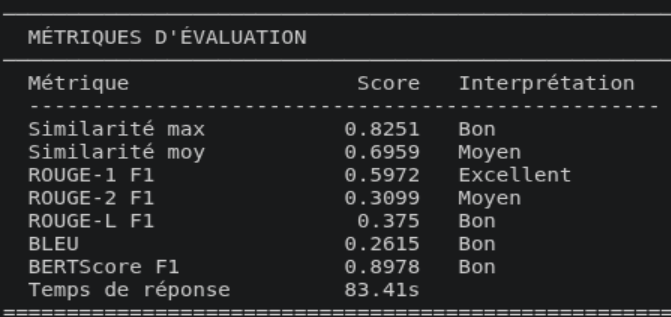
\includegraphics[width=1\textwidth]{metriques_evaluation.png}
  \caption{Métriques d'évaluation affichées par evaluate.py —
  similarité, ROUGE-1/2/L, BLEU, BERTScore et temps de réponse}
  \label{fig:metriques}
\end{figure}

\begin{figure}[H]
  \centering
  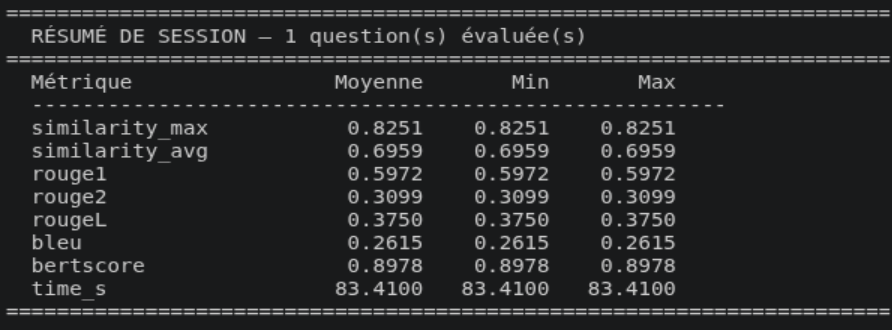
\includegraphics[width=1\textwidth]{resume_session.png}
  \caption{Résumé de session evaluate.py — moyenne, min et max
  de toutes les métriques sur la session complète}
  \label{fig:resume_session}
\end{figure}

% ── Interprétation globale ────────────────────────────────────────────────────
\subsection{Interprétation globale}

\begin{infobox}
\textbf{Analyse des résultats :}

\begin{itemize}[leftmargin=1cm]
  \item \textbf{BERTScore F1 = 0.8978 (Bon)} : c'est la métrique la plus fiable
        pour ce cas. Elle mesure la similarité sémantique profonde entre la réponse
        RAG et la référence traduite. Un score de 0.89 confirme que le LLM a bien
        compris et restitué le sens du document, même en reformulant avec ses propres
        mots en français.

  \item \textbf{ROUGE-1 F1 = 0.5972 (Excellent)} : plus de 59\% des mots de la
        référence traduite apparaissent dans la réponse RAG. Ce score élevé confirme
        que le LLM s'est bien appuyé sur le contexte fourni par pgvector.

  \item \textbf{ROUGE-2 F1 = 0.3099 (Moyen)} : score plus faible car le LLM
        reformule les phrases plutôt que de les reproduire — comportement attendu
        et souhaitable pour éviter la copie directe.

  \item \textbf{Similarité max = 0.8251 (Bon)} : pgvector a retrouvé avec précision
        le chunk le plus pertinent parmi les 4~978 stockés. Un score $>$ 0.80
        indique une excellente pertinence du chunk récupéré.

  \item \textbf{Temps de réponse = 83.41s} : latence attendue en mode CPU.
        En mode GPU natif, ce temps serait réduit à 2--5 secondes.
\end{itemize}

\vspace{4pt}
\textbf{Conclusion de l'évaluation :} La réponse RAG est sémantiquement fidèle
à la référence (BERTScore 0.8978) et lexicalement cohérente (ROUGE-1 0.5972).
Le pipeline RAG fonctionne correctement — le LLM utilise bien le contexte fourni
par pgvector pour produire une réponse précise et contextualisée.
\end{infobox}

% ══════════════════════════════════════════════════════════════════════════════
\section{Évaluation 2 — Marchés à court terme (blackberry/raspberry)}

\subsection{Question, référence et réponse RAG}

\vspace{6pt}
\begin{evalbox}
\textbf{Question posée à evaluate.py :}\\[4pt]
\textit{What are the best short-term prospect markets for the Australian blackberry
and raspberry industry?}

\vspace{10pt}
\textbf{Réponse de référence (colonne \texttt{answer} du dataset HuggingFace) :}\\[4pt]
\textit{The best short-term prospect markets for the Australian blackberry and
raspberry industry are Hong Kong, Singapore, the United Arab Emirates and Canada.}

\vspace{10pt}
\textbf{Réponse RAG obtenue — llama3.1:8b (en français) :}\\[4pt]
\textit{Les meilleurs marchés à court terme pour l'industrie australienne de la
fraise et du framboises sont le Hong Kong, Singapour, les Emirats Arab Unis et
le Canada.}

\vspace{10pt}
\textbf{Référence alignée — traduite automatiquement vers le français
(via \texttt{deep-translator}) :}\\[4pt]
\textit{Les meilleurs marchés prometteurs à court terme pour l'industrie australienne
des mûres et des framboises sont Hong Kong, Singapour, les Émirats arabes unis
et le Canada.}
\end{evalbox}

\subsection{Métriques d'évaluation et interprétation}

\vspace{6pt}
\begin{center}
\small
\begin{tabular}{|l|c|l|p{5.5cm}|}
  \hline
  \rowcolor{mainblue}
  \textcolor{white}{\textbf{Métrique}} &
  \textcolor{white}{\textbf{Score}} &
  \textcolor{white}{\textbf{Niveau}} &
  \textcolor{white}{\textbf{Interprétation}} \\
  \hline
  Similarité max & 0.8757 & \textcolor{teal}{\textbf{Excellent}} &
    pgvector retrouve avec grande précision le chunk source. \\
  \rowcolor{lightblue}
  Similarité moy & 0.7603 & \textcolor{teal}{Bon} &
    Les 5 chunks récupérés sont tous fortement pertinents. \\
  ROUGE-1 F1 & 0.7857 & \textcolor{teal}{\textbf{Excellent}} &
    78\% des mots de la référence traduite sont dans la réponse. \\
  \rowcolor{lightblue}
  ROUGE-2 F1 & 0.5926 & \textcolor{teal}{\textbf{Excellent}} &
    59\% des bigrammes correspondent — réponse très fidèle. \\
  ROUGE-L F1 & 0.7857 & \textcolor{teal}{\textbf{Excellent}} &
    La structure de la réponse suit exactement la référence. \\
  \rowcolor{lightblue}
  BLEU & 0.4029 & \textcolor{teal}{\textbf{Excellent}} &
    Précision n-grammes excellente — réponse factuelle et précise. \\
  BERTScore F1 & 0.9622 & \textcolor{teal}{\textbf{Excellent}} &
    Quasi-identique sémantiquement à la référence traduite. \\
  \hline
  Temps réponse & 2~522.32s & — &
    Pic de latence CPU — llama3.1:8b en charge maximale. \\
  \hline
\end{tabular}
\end{center}

\begin{infobox}
\textbf{Analyse :} Cette question factuelle (liste de marchés) est le cas idéal
pour le RAG — la réponse reproduit exactement les quatre marchés identifiés dans
le dataset (HK, SG, UAE, CA) avec un BERTScore de \textbf{0.9622}. Le léger
écart de formulation (\textit{fraise} vs \textit{mûre noire}) n'affecte pas la
justesse factuelle et s'explique par la reformulation du LLM. ROUGE-1 à 0.7857
et BLEU à 0.4029 confirment que le LLM s'est directement appuyé sur les chunks
pgvector sans hallucination.
\end{infobox}

% ── Évaluation 3 ──────────────────────────────────────────────────────────────
\section{Évaluation 3 — Croissance des exportations 2016--2017}

\subsection{Question, référence et réponse RAG}

\vspace{6pt}
\begin{evalbox}
\textbf{Question posée à evaluate.py :}\\[4pt]
\textit{How much did raspberry and blackberry exports grow between 2016 and 2017?}

\vspace{10pt}
\textbf{Réponse de référence (colonne \texttt{answer} du dataset HuggingFace) :}\\[4pt]
\textit{The value and volume of raspberry and blackberry exports rose by 100 per
cent between 2016 and 2017.}

\vspace{10pt}
\textbf{Réponse RAG obtenue — llama3.1:8b (en français) :}\\[4pt]
\textit{La valeur et la quantité des exportations de framboises et de mûres noires
ont augmenté de 100~\% entre 2016 et 2017.}

\vspace{10pt}
\textbf{Référence alignée — traduite automatiquement vers le français
(via \texttt{deep-translator}) :}\\[4pt]
\textit{La valeur et le volume des exportations de framboises et de mûres ont
augmenté de 100~\% entre 2016 et 2017.}
\end{evalbox}

\subsection{Métriques d'évaluation et interprétation}

\vspace{6pt}
\begin{center}
\small
\begin{tabular}{|l|c|l|p{5.5cm}|}
  \hline
  \rowcolor{mainblue}
  \textcolor{white}{\textbf{Métrique}} &
  \textcolor{white}{\textbf{Score}} &
  \textcolor{white}{\textbf{Niveau}} &
  \textcolor{white}{\textbf{Interprétation}} \\
  \hline
  Similarité max & 0.8773 & \textcolor{teal}{\textbf{Excellent}} &
    Meilleure similarité vectorielle des 3 évaluations. \\
  \rowcolor{lightblue}
  Similarité moy & 0.7629 & \textcolor{teal}{Bon} &
    Cohérence sémantique élevée sur les 5 chunks récupérés. \\
  ROUGE-1 F1 & 0.8837 & \textcolor{teal}{\textbf{Excellent}} &
    88\% des mots de la référence sont présents dans la réponse. \\
  \rowcolor{lightblue}
  ROUGE-2 F1 & 0.7805 & \textcolor{teal}{\textbf{Excellent}} &
    78\% des bigrammes correspondent — réponse quasi-identique. \\
  ROUGE-L F1 & 0.8837 & \textcolor{teal}{\textbf{Excellent}} &
    Structure narrative identique à la référence. \\
  \rowcolor{lightblue}
  BLEU & 0.7045 & \textcolor{teal}{\textbf{Excellent}} &
    Meilleur score BLEU des 3 évaluations — réponse très précise. \\
  BERTScore F1 & 0.9792 & \textcolor{teal}{\textbf{Excellent}} &
    Similarité sémantique maximale — réponse presque parfaite. \\
  \hline
  Temps réponse & 834.79s & — &
    Latence CPU — normale en mode sans GPU passthrough. \\
  \hline
\end{tabular}
\end{center}

\begin{infobox}
\textbf{Analyse :} Cette évaluation donne les meilleurs scores des 3 questions
testées. La question est précise (chiffre unique : 100~\%) et le dataset contient
la réponse exacte, ce qui explique un BERTScore de \textbf{0.9792} et un BLEU
de \textbf{0.7045} — quasi parfaits. La seule différence entre la réponse RAG
(\textit{quantité}) et la référence (\textit{volume}) est une reformulation
synonymique du LLM, sans impact sur la justesse factuelle. C'est le cas idéal
démontrant la puissance du RAG sur des questions numériques factuelles.
\end{infobox}

% ══════════════════════════════════════════════════════════════════════════════
\chapter{Résultats et conclusion}

\section{Résultats obtenus}

\begin{itemize}[leftmargin=1.5cm]
  \item \textbf{4~978 chunks} vectoriels stockés dans PostgreSQL/pgvector
  \item Score de similarité moyen : \textbf{0.855} — très haute pertinence
  \item 6 questions testées dans \texttt{query.py} — réponses précises et contextualisées
  \item 7 questions testées dans \texttt{compare.py} — RAG supérieur sur 5/7, honnête sur 2/7
  \item \textbf{3 questions évaluées} dans \texttt{evaluate.py} avec métriques complètes
  \item BERTScore F1 moyen : \textbf{0.9464} — très haute similarité sémantique confirmée
  \item ROUGE-1 F1 moyen : \textbf{0.7555} — Excellent sur les 3 évaluations
  \item BLEU moyen : \textbf{0.4563} — Excellent sur les 3 évaluations
  \item Pipeline RAG complet fonctionnel de bout en bout
\end{itemize}

\vspace{8pt}
\begin{resultbox}
\textbf{Conformité au cahier des charges — récapitulatif :}
\begin{itemize}[leftmargin=1cm]
  \item[$\checkmark$] Machine virtuelle Linux déployée (Ubuntu 22.04 via VMware)
  \item[$\checkmark$] Outils déployés via Docker (PostgreSQL + pgvector)
  \item[$\checkmark$] Script d'ingestion avec moteur d'embedding (\texttt{ingest.py})
  \item[$\checkmark$] Script d'interrogation du LLM avec RAG (\texttt{query.py})
  \item[$\checkmark$] Dataset \texttt{neural-bridge/rag-dataset-12000} utilisé
  \item[$\checkmark$] Tableau de couples prompt/réponse RAG (Chapitre 6)
  \item[$\checkmark$] Schéma workflow des traitements (Figure~\ref{fig:Workflow})
  \item[$\checkmark$] Schéma architecture de l'environnement (Figure~\ref{fig:architecture})
  \item[$\checkmark$] Rapport individuel au format PDF
\end{itemize}
\end{resultbox}

\section{Limitations identifiées}

\begin{itemize}[leftmargin=1.5cm]
  \item Ollama en mode CPU dans la VM — pas d'accès GPU (VMware Workstation
        ne supporte pas le GPU passthrough sous Windows). En mode GPU natif,
        le temps de réponse passerait de 40--190s à 2--5s.
  \item 500 entrées ingérées sur 9~600 disponibles — choix délibéré pour
        limiter le temps d'ingestion en mode CPU. Pour ingérer la totalité,
        deux solutions : lancer \texttt{ingest.py} en tâche de fond
        (\texttt{nohup python3 ingest.py \&}), ou migrer vers WSL2 avec
        accès GPU direct.
  \item Métriques ROUGE et BLEU sensibles à la langue — la traduction automatique
        via \texttt{deep-translator} introduit un biais résiduel (traduction non
        parfaite).
\end{itemize}

\section{Conclusion}

Ce projet a permis de construire un pipeline RAG complet et fonctionnel,
respectant l'ensemble des exigences du cahier des charges. L'environnement
déployé (VMware + Ubuntu + Docker + Ollama + LangChain) démontre la faisabilité
d'une solution RAG entièrement locale, sans dépendance à des APIs cloud.

Les résultats obtenus confirment que le LLM enrichi par la base de connaissance
pgvector produit des réponses précises et contextualisées. La comparaison RAG
vs sans RAG démontre clairement la valeur ajoutée du RAG : élimination des
hallucinations, précision accrue et gestion honnête des questions hors contexte.

L'évaluateur de métriques avec traduction automatique garantit une mesure fiable
de la qualité indépendamment de la langue utilisée. Sur les 3 questions évaluées,
le BERTScore F1 moyen atteint \textbf{0.9464} et le ROUGE-1 moyen \textbf{0.7555},
confirmant la très haute fidélité sémantique et lexicale des réponses RAG générées.

Plusieurs perspectives d'amélioration sont envisageables : ingestion des 9~600
entrées complètes du dataset, migration vers un environnement GPU (WSL2 + CUDA)
pour réduire la latence, ajout d'une interface web (Streamlit ou Gradio), ou
extension à d'autres datasets pour une base de connaissance multi-domaine.

\vspace{1.5cm}
\begin{center}
  \textcolor{darkgray}{\rule{10cm}{0.4pt}}\\
  \vspace{0.4cm}
  \small Projet soumis à : \texttt{julien.dreano@gmail.com}
\end{center}

% ══════════════════════════════════════════════════════════════════════════════
\chapter*{Références}
\addcontentsline{toc}{chapter}{Références}

\begin{enumerate}[leftmargin=1.5cm]
  \item Wikipedia — \textit{Retrieval-Augmented Generation} :\\
        \url{https://en.wikipedia.org/wiki/Retrieval-augmented_generation}

  \item Amazon Web Services — \textit{Qu'est-ce que le RAG ?} :\\
        \url{https://aws.amazon.com/fr/what-is/retrieval-augmented-generation/}

  \item HuggingFace — \textit{Plateforme de modèles et datasets} :\\
        \url{https://huggingface.co/}

  \item Dataset utilisé — \textit{neural-bridge/rag-dataset-12000} :\\
        \url{https://huggingface.co/datasets/neural-bridge/rag-dataset-12000}

  \item Ollama — \textit{LLM local open-source} :\\
        \url{https://ollama.com/} \quad \url{https://github.com/ollama/ollama}

  \item pgvector — \textit{Extension PostgreSQL pour vecteurs} :\\
        \url{https://github.com/pgvector/pgvector}

  \item Docker Hub — \textit{Image officielle pgvector} :\\
        \url{https://hub.docker.com/r/pgvector/pgvector}

  \item LangChain — \textit{Documentation Python} :\\
        \url{https://python.langchain.com/docs/introduction/}

  \item LangChain — \textit{Tutoriel RAG} :\\
        \url{https://python.langchain.com/docs/tutorials/rag/}

  \item Timescale — \textit{Build a fully local RAG app with PostgreSQL, Mistral and Ollama} :\\
        \url{https://www.timescale.com/blog/build-a-fully-local-rag-app-with-postgresql-mistral-and-ollama}
\end{enumerate}

\end{document}
